% Options for packages loaded elsewhere
\PassOptionsToPackage{unicode}{hyperref}
\PassOptionsToPackage{hyphens}{url}
\PassOptionsToPackage{dvipsnames,svgnames,x11names}{xcolor}
%
\documentclass[
  letterpaper,
  DIV=11,
  numbers=noendperiod]{scrartcl}

\usepackage{amsmath,amssymb}
\usepackage{iftex}
\ifPDFTeX
  \usepackage[T1]{fontenc}
  \usepackage[utf8]{inputenc}
  \usepackage{textcomp} % provide euro and other symbols
\else % if luatex or xetex
  \usepackage{unicode-math}
  \defaultfontfeatures{Scale=MatchLowercase}
  \defaultfontfeatures[\rmfamily]{Ligatures=TeX,Scale=1}
\fi
\usepackage{lmodern}
\ifPDFTeX\else  
    % xetex/luatex font selection
\fi
% Use upquote if available, for straight quotes in verbatim environments
\IfFileExists{upquote.sty}{\usepackage{upquote}}{}
\IfFileExists{microtype.sty}{% use microtype if available
  \usepackage[]{microtype}
  \UseMicrotypeSet[protrusion]{basicmath} % disable protrusion for tt fonts
}{}
\makeatletter
\@ifundefined{KOMAClassName}{% if non-KOMA class
  \IfFileExists{parskip.sty}{%
    \usepackage{parskip}
  }{% else
    \setlength{\parindent}{0pt}
    \setlength{\parskip}{6pt plus 2pt minus 1pt}}
}{% if KOMA class
  \KOMAoptions{parskip=half}}
\makeatother
\usepackage{xcolor}
\usepackage[margin=1.3cm]{geometry}
\setlength{\emergencystretch}{3em} % prevent overfull lines
\setcounter{secnumdepth}{5}
% Make \paragraph and \subparagraph free-standing
\makeatletter
\ifx\paragraph\undefined\else
  \let\oldparagraph\paragraph
  \renewcommand{\paragraph}{
    \@ifstar
      \xxxParagraphStar
      \xxxParagraphNoStar
  }
  \newcommand{\xxxParagraphStar}[1]{\oldparagraph*{#1}\mbox{}}
  \newcommand{\xxxParagraphNoStar}[1]{\oldparagraph{#1}\mbox{}}
\fi
\ifx\subparagraph\undefined\else
  \let\oldsubparagraph\subparagraph
  \renewcommand{\subparagraph}{
    \@ifstar
      \xxxSubParagraphStar
      \xxxSubParagraphNoStar
  }
  \newcommand{\xxxSubParagraphStar}[1]{\oldsubparagraph*{#1}\mbox{}}
  \newcommand{\xxxSubParagraphNoStar}[1]{\oldsubparagraph{#1}\mbox{}}
\fi
\makeatother

\usepackage{color}
\usepackage{fancyvrb}
\newcommand{\VerbBar}{|}
\newcommand{\VERB}{\Verb[commandchars=\\\{\}]}
\DefineVerbatimEnvironment{Highlighting}{Verbatim}{commandchars=\\\{\}}
% Add ',fontsize=\small' for more characters per line
\usepackage{framed}
\definecolor{shadecolor}{RGB}{241,243,245}
\newenvironment{Shaded}{\begin{snugshade}}{\end{snugshade}}
\newcommand{\AlertTok}[1]{\textcolor[rgb]{0.68,0.00,0.00}{#1}}
\newcommand{\AnnotationTok}[1]{\textcolor[rgb]{0.37,0.37,0.37}{#1}}
\newcommand{\AttributeTok}[1]{\textcolor[rgb]{0.40,0.45,0.13}{#1}}
\newcommand{\BaseNTok}[1]{\textcolor[rgb]{0.68,0.00,0.00}{#1}}
\newcommand{\BuiltInTok}[1]{\textcolor[rgb]{0.00,0.23,0.31}{#1}}
\newcommand{\CharTok}[1]{\textcolor[rgb]{0.13,0.47,0.30}{#1}}
\newcommand{\CommentTok}[1]{\textcolor[rgb]{0.37,0.37,0.37}{#1}}
\newcommand{\CommentVarTok}[1]{\textcolor[rgb]{0.37,0.37,0.37}{\textit{#1}}}
\newcommand{\ConstantTok}[1]{\textcolor[rgb]{0.56,0.35,0.01}{#1}}
\newcommand{\ControlFlowTok}[1]{\textcolor[rgb]{0.00,0.23,0.31}{\textbf{#1}}}
\newcommand{\DataTypeTok}[1]{\textcolor[rgb]{0.68,0.00,0.00}{#1}}
\newcommand{\DecValTok}[1]{\textcolor[rgb]{0.68,0.00,0.00}{#1}}
\newcommand{\DocumentationTok}[1]{\textcolor[rgb]{0.37,0.37,0.37}{\textit{#1}}}
\newcommand{\ErrorTok}[1]{\textcolor[rgb]{0.68,0.00,0.00}{#1}}
\newcommand{\ExtensionTok}[1]{\textcolor[rgb]{0.00,0.23,0.31}{#1}}
\newcommand{\FloatTok}[1]{\textcolor[rgb]{0.68,0.00,0.00}{#1}}
\newcommand{\FunctionTok}[1]{\textcolor[rgb]{0.28,0.35,0.67}{#1}}
\newcommand{\ImportTok}[1]{\textcolor[rgb]{0.00,0.46,0.62}{#1}}
\newcommand{\InformationTok}[1]{\textcolor[rgb]{0.37,0.37,0.37}{#1}}
\newcommand{\KeywordTok}[1]{\textcolor[rgb]{0.00,0.23,0.31}{\textbf{#1}}}
\newcommand{\NormalTok}[1]{\textcolor[rgb]{0.00,0.23,0.31}{#1}}
\newcommand{\OperatorTok}[1]{\textcolor[rgb]{0.37,0.37,0.37}{#1}}
\newcommand{\OtherTok}[1]{\textcolor[rgb]{0.00,0.23,0.31}{#1}}
\newcommand{\PreprocessorTok}[1]{\textcolor[rgb]{0.68,0.00,0.00}{#1}}
\newcommand{\RegionMarkerTok}[1]{\textcolor[rgb]{0.00,0.23,0.31}{#1}}
\newcommand{\SpecialCharTok}[1]{\textcolor[rgb]{0.37,0.37,0.37}{#1}}
\newcommand{\SpecialStringTok}[1]{\textcolor[rgb]{0.13,0.47,0.30}{#1}}
\newcommand{\StringTok}[1]{\textcolor[rgb]{0.13,0.47,0.30}{#1}}
\newcommand{\VariableTok}[1]{\textcolor[rgb]{0.07,0.07,0.07}{#1}}
\newcommand{\VerbatimStringTok}[1]{\textcolor[rgb]{0.13,0.47,0.30}{#1}}
\newcommand{\WarningTok}[1]{\textcolor[rgb]{0.37,0.37,0.37}{\textit{#1}}}

\providecommand{\tightlist}{%
  \setlength{\itemsep}{0pt}\setlength{\parskip}{0pt}}\usepackage{longtable,booktabs,array}
\usepackage{calc} % for calculating minipage widths
% Correct order of tables after \paragraph or \subparagraph
\usepackage{etoolbox}
\makeatletter
\patchcmd\longtable{\par}{\if@noskipsec\mbox{}\fi\par}{}{}
\makeatother
% Allow footnotes in longtable head/foot
\IfFileExists{footnotehyper.sty}{\usepackage{footnotehyper}}{\usepackage{footnote}}
\makesavenoteenv{longtable}
\usepackage{graphicx}
\makeatletter
\def\maxwidth{\ifdim\Gin@nat@width>\linewidth\linewidth\else\Gin@nat@width\fi}
\def\maxheight{\ifdim\Gin@nat@height>\textheight\textheight\else\Gin@nat@height\fi}
\makeatother
% Scale images if necessary, so that they will not overflow the page
% margins by default, and it is still possible to overwrite the defaults
% using explicit options in \includegraphics[width, height, ...]{}
\setkeys{Gin}{width=\maxwidth,height=\maxheight,keepaspectratio}
% Set default figure placement to htbp
\makeatletter
\def\fps@figure{htbp}
\makeatother
% definitions for citeproc citations
\NewDocumentCommand\citeproctext{}{}
\NewDocumentCommand\citeproc{mm}{%
  \begingroup\def\citeproctext{#2}\cite{#1}\endgroup}
\makeatletter
 % allow citations to break across lines
 \let\@cite@ofmt\@firstofone
 % avoid brackets around text for \cite:
 \def\@biblabel#1{}
 \def\@cite#1#2{{#1\if@tempswa , #2\fi}}
\makeatother
\newlength{\cslhangindent}
\setlength{\cslhangindent}{1.5em}
\newlength{\csllabelwidth}
\setlength{\csllabelwidth}{3em}
\newenvironment{CSLReferences}[2] % #1 hanging-indent, #2 entry-spacing
 {\begin{list}{}{%
  \setlength{\itemindent}{0pt}
  \setlength{\leftmargin}{0pt}
  \setlength{\parsep}{0pt}
  % turn on hanging indent if param 1 is 1
  \ifodd #1
   \setlength{\leftmargin}{\cslhangindent}
   \setlength{\itemindent}{-1\cslhangindent}
  \fi
  % set entry spacing
  \setlength{\itemsep}{#2\baselineskip}}}
 {\end{list}}
\usepackage{calc}
\newcommand{\CSLBlock}[1]{\hfill\break\parbox[t]{\linewidth}{\strut\ignorespaces#1\strut}}
\newcommand{\CSLLeftMargin}[1]{\parbox[t]{\csllabelwidth}{\strut#1\strut}}
\newcommand{\CSLRightInline}[1]{\parbox[t]{\linewidth - \csllabelwidth}{\strut#1\strut}}
\newcommand{\CSLIndent}[1]{\hspace{\cslhangindent}#1}

\usepackage{ragged2e}
\justifying
\KOMAoption{captions}{tableheading}
\makeatletter
\@ifpackageloaded{caption}{}{\usepackage{caption}}
\AtBeginDocument{%
\ifdefined\contentsname
  \renewcommand*\contentsname{Table of contents}
\else
  \newcommand\contentsname{Table of contents}
\fi
\ifdefined\listfigurename
  \renewcommand*\listfigurename{List of Figures}
\else
  \newcommand\listfigurename{List of Figures}
\fi
\ifdefined\listtablename
  \renewcommand*\listtablename{List of Tables}
\else
  \newcommand\listtablename{List of Tables}
\fi
\ifdefined\figurename
  \renewcommand*\figurename{Figure}
\else
  \newcommand\figurename{Figure}
\fi
\ifdefined\tablename
  \renewcommand*\tablename{Table}
\else
  \newcommand\tablename{Table}
\fi
}
\@ifpackageloaded{float}{}{\usepackage{float}}
\floatstyle{ruled}
\@ifundefined{c@chapter}{\newfloat{codelisting}{h}{lop}}{\newfloat{codelisting}{h}{lop}[chapter]}
\floatname{codelisting}{Listing}
\newcommand*\listoflistings{\listof{codelisting}{List of Listings}}
\makeatother
\makeatletter
\makeatother
\makeatletter
\@ifpackageloaded{caption}{}{\usepackage{caption}}
\@ifpackageloaded{subcaption}{}{\usepackage{subcaption}}
\makeatother

\ifLuaTeX
  \usepackage{selnolig}  % disable illegal ligatures
\fi
\usepackage{bookmark}

\IfFileExists{xurl.sty}{\usepackage{xurl}}{} % add URL line breaks if available
\urlstyle{same} % disable monospaced font for URLs
\hypersetup{
  pdftitle={HARVARD EXTENSION SCHOOL},
  pdfauthor={Author: Dinesh Bedathuru; Author: Brian Calderon; Author: Jeisson Hernandez; Author: Hao Fu; Author: Derek Rush; Author: Jeremy Tajonera; Author: Catherine Tully},
  colorlinks=true,
  linkcolor={blue},
  filecolor={Maroon},
  citecolor={Blue},
  urlcolor={Blue},
  pdfcreator={LaTeX via pandoc}}


\title{HARVARD EXTENSION SCHOOL}
\usepackage{etoolbox}
\makeatletter
\providecommand{\subtitle}[1]{% add subtitle to \maketitle
  \apptocmd{\@title}{\par {\large #1 \par}}{}{}
}
\makeatother
\subtitle{EXT CSCI E-106 Model Data Class Group Project Template}
\author{Author: Dinesh Bedathuru \and Author: Brian
Calderon \and Author: Jeisson Hernandez \and Author: Hao Fu \and Author:
Derek Rush \and Author: Jeremy Tajonera \and Author: Catherine Tully}
\date{06 May 2025}

\begin{document}
\maketitle
\begin{abstract}
In this project, our aim is to classify the probability of a passenger
surviving the Titanic crash of 1912. We used a variety of linear and
non-linear models to deduce the most accurate model and provide
long-term stability in our predictions.
\end{abstract}

\renewcommand*\contentsname{Table of contents}
{
\hypersetup{linkcolor=}
\setcounter{tocdepth}{2}
\tableofcontents
}
\listoffigures
\listoftables

Classify whether a passenger on board the maiden voyage of the RMS
Titanic in 1912 survived given their age, sex and class.
Sample-Data-Titanic-Survival.csv to be used in the Final Project

\begin{longtable}[]{@{}
  >{\raggedright\arraybackslash}p{(\columnwidth - 2\tabcolsep) * \real{0.5000}}
  >{\raggedright\arraybackslash}p{(\columnwidth - 2\tabcolsep) * \real{0.5000}}@{}}
\toprule\noalign{}
\begin{minipage}[b]{\linewidth}\raggedright
Variable
\end{minipage} & \begin{minipage}[b]{\linewidth}\raggedright
Description
\end{minipage} \\
\midrule\noalign{}
\endhead
\bottomrule\noalign{}
\endlastfoot
pclass & \textbf{Passenger Class (1 = 1st; 2 = 2nd; 3 = 3rd)} \\
survived & \textbf{Survival (0 = No; 1 = Yes)} \\
name & \textbf{Name} \\
sex & \textbf{Sex} \\
age & \textbf{Age} \\
sibsp & \textbf{\# of siblings / spouses aboard the Titanic} \\
parch & \textbf{\# of parents / children aboard the Titanic} \\
ticket & \textbf{Ticket number} \\
fare & \textbf{Passenger fare} \\
cabin & \textbf{Cabin number} \\
embarked & \textbf{Port of Embarkation (C = Cherbourg; Q = Queenstown; S
= Southampton)} \\
boat & \textbf{Lifeboat ID, if passenger survived} \\
body & \textbf{Body number (if passenger did not survive and body was
recovered} \\
home.dest & \textbf{The intended home destination of the passenger} \\
\end{longtable}

\section{Instructions:}\label{instructions}

0. Join a team with your fellow students with appropriate size (Up to
Nine Students total) If you have not group by the end of the week of
April 11 you may present the project by yourself or I will randomly
assign other stranded student to your group. I will let know the final
groups in April 11.

1. Load and Review the dataset named ``Titanic\_Survival\_Data.csv'' 2.
Create the train data set which contains 70\% of the data and use
set.seed (15). The remaining 30\% will be your test data set.

3. Investigate the data and combine the level of categorical variables
if needed and drop variables as needed. For example, you can drop id,
Latitude, Longitude, etc.

4. Build appropriate model to predict the probability of survival.

5. Create scatter plots and a correlation matrix for the train data set.
Interpret the possible relationship between the response.

6. Build the best models by using the appropriate selection method.
Compare the performance of the best logistic linear models.

7. Make sure that model assumption(s) are checked for the final model.
Apply remedy measures (transformation, etc.) that helps satisfy the
assumptions.

8. Investigate unequal variances and multicollinearity.

9. Build an alternative to your model based on one of the following
approaches as applicable to predict the probability of survival:
logistic regression, classification Tree, NN, or SVM. Check the
applicable model assumptions. Explore using a negative binomial
regression and a Poisson regression.

10. Use the test data set to assess the model performances from above.

11. Based on the performances on both train and test data sets,
determine your primary (champion) model and the other model which would
be your benchmark model.

12. Create a model development document that describes the model
following this template, input the name of the authors, Harvard IDs, the
name of the Group, all of your code and calculations, etc..

\textbf{Due Date: May 12 2025 1159 pm hours EST Notes No typographical
errors, grammar mistakes, or misspelled words, use English language All
tables need to be numbered and describe their content in the body of the
document All figures/graphs need to be numbered and describe their
content All results must be accurate and clearly explained for a casual
reviewer to fully understand their purpose and impact Submit both the
RMD markdown file and PDF with the sections with appropriate
explanations. A more formal.}

\section{Executive Summary}\label{executive-summary}

This section will describe the model usage, your conclusions and any
regulatory and internal requirements. In a real world scneario, this
section is for senior management who do not need to know the details.
They need to know high level (the purpose of the model, limitations of
the model and any issues).

\section{I. Introduction (5 points)}\label{i.-introduction-5-points}

This section needs to introduce the reader to the problem to be
resolved, the purpose, and the scope of the statistical testing applied.
What you are doing with your prediction? What is the purpose of the
model? What methods were trained on the data, how large is the test
sample, and how did you build the model?

The Titanic was a British-registered ship that set sail on its maiden
voyage on April 10th, 1912 with 2,240 passengers and crew on board. On
April 15th, 1912, the ship struck an iceberg, split in half, and sank to
the bottom of the ocean (National Oceanic and Atmospheric Administration
(NOAA), 2023). In this report, we are going to analyze the data in the
Titanic.csv file and use it to determine the best model for predicting
whether someone on board would live or die. By creating this model, we
hope to understand what factors a passenger could have taken into
account in order to reduce their risk of death during the trip. We
cleaned the data and split into into a train/test split in order to
properly train our models. We created simple linear models, multivariate
linear models, logistic models (both binomial and poisson), a regression
tree, and a neural network model. The train sample size was 916 data
points (70.03\%) and the test sample size was 392 data points (29.97\%).
We built the models after examining the data and determining which
predictor variables we thought would be most relevant for survival rate.
Once we had our variables and training data, we created the models and
examined the performance of the models on both training and testing data
to determine if they were robust. We also examined if the model
assumptions appeared to hold for each model.

\section{II. Description of the data and
quality}\label{ii.-description-of-the-data-and-quality}

Here you need to review your data, the statistical test applied to
understand the predictors and the response and how are they correlated.
Extensive graph analysis is recommended. Is the data continuous, or
categorical, do any transformation needed? Do you need dummies?

\subsection{Loading the data}\label{loading-the-data}

\begin{Shaded}
\begin{Highlighting}[]
\NormalTok{odata }\OtherTok{\textless{}{-}} \FunctionTok{read.csv}\NormalTok{(}\StringTok{"../data/Titanic\_Survival\_Data.csv"}\NormalTok{)}
\FunctionTok{cat}\NormalTok{(}\StringTok{"Size of entire data set:"}\NormalTok{, }\FunctionTok{nrow}\NormalTok{(odata), }\StringTok{"}\SpecialCharTok{\textbackslash{}n}\StringTok{"}\NormalTok{)}
\end{Highlighting}
\end{Shaded}

\begin{verbatim}
Size of entire data set: 1310 
\end{verbatim}

\subsection{Removing un-needed
columns}\label{removing-un-needed-columns}

Name: Removing because names have no inference on surivival (inference)

ticket: Ticket No.~will also likely not have an influence in survival

boat: This is highly correlated to the survival dependant variable since
people who made it on a boat likely survived

body: This is highly correlated to the survival dependant variable since
people who's body was recovered did not survive.

home.dest: The destination likely has nothing to do with the survival

\begin{Shaded}
\begin{Highlighting}[]
\NormalTok{data.clean }\OtherTok{=}\NormalTok{ odata[, }\SpecialCharTok{!}\NormalTok{(}\FunctionTok{names}\NormalTok{(odata) }\SpecialCharTok{\%in\%} \FunctionTok{c}\NormalTok{(}\StringTok{"name"}\NormalTok{, }\StringTok{"ticket"}\NormalTok{, }\StringTok{"boat"}\NormalTok{,}\StringTok{"body"}\NormalTok{,}\StringTok{"home.dest"}\NormalTok{))]}
\end{Highlighting}
\end{Shaded}

\subsection{Data Augmentation}\label{data-augmentation}

We extracted the deck letter from the cabin since it could potentially
correlate to the survival.

\begin{Shaded}
\begin{Highlighting}[]
\CommentTok{\#Extract deck letter from cabin}
\NormalTok{data.clean}\SpecialCharTok{$}\NormalTok{deck }\OtherTok{\textless{}{-}} \FunctionTok{substr}\NormalTok{(data.clean}\SpecialCharTok{$}\NormalTok{cabin, }\DecValTok{1}\NormalTok{,}\DecValTok{1}\NormalTok{)}
\CommentTok{\# Remove cabin col:}
\NormalTok{data.clean}\SpecialCharTok{$}\NormalTok{cabin }\OtherTok{\textless{}{-}} \ConstantTok{NULL}
\end{Highlighting}
\end{Shaded}

\subsection{Initial Check for Missing
values}\label{initial-check-for-missing-values}

We see that age and deck have the most amount of missing data, therefore
we proceed to impute them.

\begin{figure}[H]

{\centering 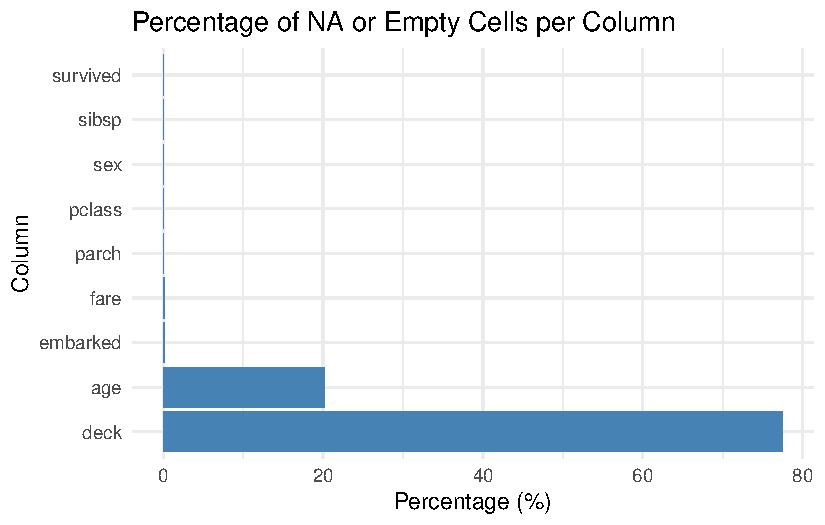
\includegraphics{FinalProject_files/figure-pdf/unnamed-chunk-4-1.pdf}

}

\caption{Percentage of Missing Values}

\end{figure}%

\subsection{Imputing data}\label{imputing-data}

Below we impute Age using the median value in that column.

For deck we use KNN to impute the missing deck values.

After imputing these two columns we can see that the largest amount of
missing data is \textasciitilde0.2\% which is quite small and can be
removed.

\begin{Shaded}
\begin{Highlighting}[]
\CommentTok{\# {-}{-}{-}{-} Age{-}{-}{-}{-}}
\CommentTok{\#Replace NAs in age column with Median value }
\NormalTok{median\_age }\OtherTok{\textless{}{-}} \FunctionTok{median}\NormalTok{(data.clean}\SpecialCharTok{$}\NormalTok{age, }\AttributeTok{na.rm =} \ConstantTok{TRUE}\NormalTok{)}
\NormalTok{data.clean }\OtherTok{\textless{}{-}}\NormalTok{ data.clean }\SpecialCharTok{\%\textgreater{}\%}
  \FunctionTok{mutate}\NormalTok{(}\AttributeTok{age =} \FunctionTok{ifelse}\NormalTok{(}\FunctionTok{is.na}\NormalTok{(age), median\_age, age))}

\CommentTok{\# {-}{-}{-}{-} deck{-}{-}{-}{-}}
\CommentTok{\# For deck, since its a category, we decided to use KNN  to impute the column:}

\CommentTok{\# Install if not already installed}
\CommentTok{\# install.packages("VIM")}
\FunctionTok{library}\NormalTok{(VIM)}
\end{Highlighting}
\end{Shaded}

\begin{verbatim}
Warning: package 'VIM' was built under R version 4.4.3
\end{verbatim}

\begin{verbatim}
Loading required package: colorspace
\end{verbatim}

\begin{verbatim}
Loading required package: grid
\end{verbatim}

\begin{verbatim}
VIM is ready to use.
\end{verbatim}

\begin{verbatim}
Suggestions and bug-reports can be submitted at: https://github.com/statistikat/VIM/issues
\end{verbatim}

\begin{verbatim}

Attaching package: 'VIM'
\end{verbatim}

\begin{verbatim}
The following object is masked from 'package:datasets':

    sleep
\end{verbatim}

\begin{Shaded}
\begin{Highlighting}[]
\CommentTok{\# Replace "" with NA in the \textquotesingle{}deck\textquotesingle{} column}
\NormalTok{data.clean}\SpecialCharTok{$}\NormalTok{deck[data.clean}\SpecialCharTok{$}\NormalTok{deck }\SpecialCharTok{==} \StringTok{""}\NormalTok{] }\OtherTok{\textless{}{-}} \ConstantTok{NA}

\CommentTok{\# Convert \textquotesingle{}cabin\textquotesingle{} to factor}
\NormalTok{data.clean}\SpecialCharTok{$}\NormalTok{deck }\OtherTok{\textless{}{-}} \FunctionTok{as.factor}\NormalTok{(data.clean}\SpecialCharTok{$}\NormalTok{deck)}

\CommentTok{\# Apply kNN imputation just to Cabin column}
\NormalTok{data.clean }\OtherTok{\textless{}{-}} \FunctionTok{kNN}\NormalTok{(data.clean, }\AttributeTok{variable =} \StringTok{"deck"}\NormalTok{, }\AttributeTok{k =} \DecValTok{5}\NormalTok{)}

\CommentTok{\# Check that NAs were imputed}
\CommentTok{\# sum(is.na(data.clean$deck))        \# Original}
\CommentTok{\# sum(is.na(data.clean.imputed$deck)) \# After}

\CommentTok{\# Remove indicator col:}
\NormalTok{data.clean}\SpecialCharTok{$}\NormalTok{deck\_imp }\OtherTok{\textless{}{-}} \ConstantTok{NULL}
\end{Highlighting}
\end{Shaded}

\begin{Shaded}
\begin{Highlighting}[]
\DocumentationTok{\#\#\#\#\#\#\#\#\#\#\#\#\#\#\#\#\#\#\#\#\#\#\#\#\#\#\#\#\#\#\#\#\#\#\#\#\#\#\#\#\#\#\#\#\#\#\#\#\#\#\#\#\#\#\#\#\#\#\#\#\#\#\#\#\#\#\#\#\#\#\#\#\#\#\#\#\#\#\#\#}
\CommentTok{\#          Check for Missing values after Imputation                           \#}
\DocumentationTok{\#\#\#\#\#\#\#\#\#\#\#\#\#\#\#\#\#\#\#\#\#\#\#\#\#\#\#\#\#\#\#\#\#\#\#\#\#\#\#\#\#\#\#\#\#\#\#\#\#\#\#\#\#\#\#\#\#\#\#\#\#\#\#\#\#\#\#\#\#\#\#\#\#\#\#\#\#\#\#\#}
\CommentTok{\# Function to calculate \% of NA or empty strings per column}
\CommentTok{\#| fig{-}cap: "Percentage of Missing Values after Imputation"}
\FunctionTok{plot\_missing\_barchart}\NormalTok{(data.clean)}
\end{Highlighting}
\end{Shaded}

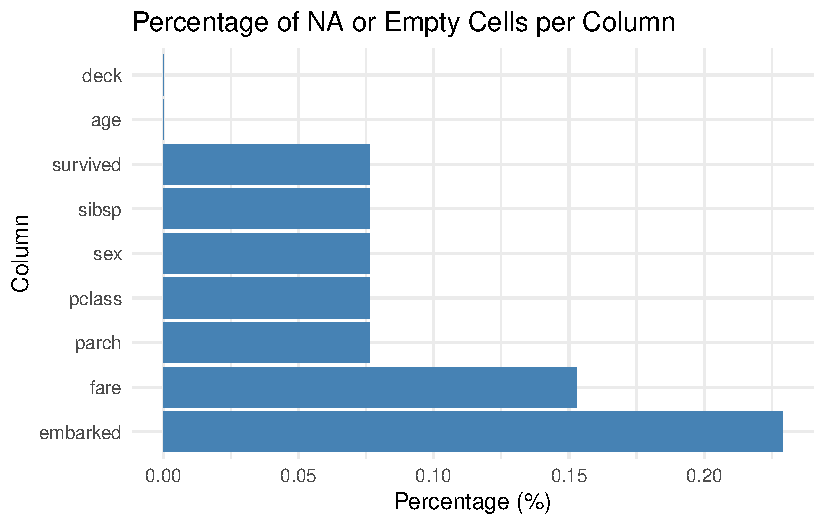
\includegraphics{FinalProject_files/figure-pdf/unnamed-chunk-6-1.pdf}

\subsection{Dummifying Columns:}\label{dummifying-columns}

We dummify pclass, sex, embarked and deck. We leave sibsp and parch as
continuous variables as we observed that dummifying these columns leads
to smaller significance, whilst leaving them as continuous maximizes
their contributions to the models explanatory power.

\begin{Shaded}
\begin{Highlighting}[]
\CommentTok{\# Dummifying pclass:}
\NormalTok{data.clean}\SpecialCharTok{$}\NormalTok{pclass\_1 }\OtherTok{=} \FunctionTok{ifelse}\NormalTok{(data.clean}\SpecialCharTok{$}\NormalTok{pclass }\SpecialCharTok{==} \DecValTok{1}\NormalTok{, }\DecValTok{1}\NormalTok{, }\DecValTok{0}\NormalTok{)}
\NormalTok{data.clean}\SpecialCharTok{$}\NormalTok{pclass\_2 }\OtherTok{=} \FunctionTok{ifelse}\NormalTok{(data.clean}\SpecialCharTok{$}\NormalTok{pclass }\SpecialCharTok{==} \DecValTok{2}\NormalTok{, }\DecValTok{1}\NormalTok{, }\DecValTok{0}\NormalTok{)}

\CommentTok{\# Dummifying sex:}
\NormalTok{data.clean}\SpecialCharTok{$}\NormalTok{sex\_M }\OtherTok{=} \FunctionTok{ifelse}\NormalTok{(data.clean}\SpecialCharTok{$}\NormalTok{sex }\SpecialCharTok{==} \StringTok{\textquotesingle{}male\textquotesingle{}}\NormalTok{, }\DecValTok{1}\NormalTok{, }\DecValTok{0}\NormalTok{)}

\CommentTok{\# Dummifying embarked:}
\NormalTok{data.clean}\SpecialCharTok{$}\NormalTok{embarked\_C }\OtherTok{=} \FunctionTok{ifelse}\NormalTok{(data.clean}\SpecialCharTok{$}\NormalTok{embarked }\SpecialCharTok{==} \StringTok{\textquotesingle{}C\textquotesingle{}}\NormalTok{, }\DecValTok{1}\NormalTok{, }\DecValTok{0}\NormalTok{)}
\NormalTok{data.clean}\SpecialCharTok{$}\NormalTok{embarked\_Q }\OtherTok{=} \FunctionTok{ifelse}\NormalTok{(data.clean}\SpecialCharTok{$}\NormalTok{embarked }\SpecialCharTok{==} \StringTok{\textquotesingle{}Q\textquotesingle{}}\NormalTok{, }\DecValTok{1}\NormalTok{, }\DecValTok{0}\NormalTok{)}

\CommentTok{\# Dummifying deck:}
\NormalTok{data.clean}\SpecialCharTok{$}\NormalTok{deck\_A }\OtherTok{=} \FunctionTok{ifelse}\NormalTok{(data.clean}\SpecialCharTok{$}\NormalTok{deck }\SpecialCharTok{==} \StringTok{\textquotesingle{}A\textquotesingle{}}\NormalTok{, }\DecValTok{1}\NormalTok{, }\DecValTok{0}\NormalTok{)}
\NormalTok{data.clean}\SpecialCharTok{$}\NormalTok{deck\_B }\OtherTok{=} \FunctionTok{ifelse}\NormalTok{(data.clean}\SpecialCharTok{$}\NormalTok{deck }\SpecialCharTok{==} \StringTok{\textquotesingle{}B\textquotesingle{}}\NormalTok{, }\DecValTok{1}\NormalTok{, }\DecValTok{0}\NormalTok{)}
\NormalTok{data.clean}\SpecialCharTok{$}\NormalTok{deck\_C }\OtherTok{=} \FunctionTok{ifelse}\NormalTok{(data.clean}\SpecialCharTok{$}\NormalTok{deck }\SpecialCharTok{==} \StringTok{\textquotesingle{}C\textquotesingle{}}\NormalTok{, }\DecValTok{1}\NormalTok{, }\DecValTok{0}\NormalTok{)}
\NormalTok{data.clean}\SpecialCharTok{$}\NormalTok{deck\_D }\OtherTok{=} \FunctionTok{ifelse}\NormalTok{(data.clean}\SpecialCharTok{$}\NormalTok{deck }\SpecialCharTok{==} \StringTok{\textquotesingle{}D\textquotesingle{}}\NormalTok{, }\DecValTok{1}\NormalTok{, }\DecValTok{0}\NormalTok{)}
\NormalTok{data.clean}\SpecialCharTok{$}\NormalTok{deck\_E }\OtherTok{=} \FunctionTok{ifelse}\NormalTok{(data.clean}\SpecialCharTok{$}\NormalTok{deck }\SpecialCharTok{==} \StringTok{\textquotesingle{}E\textquotesingle{}}\NormalTok{, }\DecValTok{1}\NormalTok{, }\DecValTok{0}\NormalTok{)}
\NormalTok{data.clean}\SpecialCharTok{$}\NormalTok{deck\_F }\OtherTok{=} \FunctionTok{ifelse}\NormalTok{(data.clean}\SpecialCharTok{$}\NormalTok{deck }\SpecialCharTok{==} \StringTok{\textquotesingle{}F\textquotesingle{}}\NormalTok{, }\DecValTok{1}\NormalTok{, }\DecValTok{0}\NormalTok{)}
\NormalTok{data.clean}\SpecialCharTok{$}\NormalTok{deck\_G }\OtherTok{=} \FunctionTok{ifelse}\NormalTok{(data.clean}\SpecialCharTok{$}\NormalTok{deck }\SpecialCharTok{==} \StringTok{\textquotesingle{}G\textquotesingle{}}\NormalTok{, }\DecValTok{1}\NormalTok{, }\DecValTok{0}\NormalTok{)}

\CommentTok{\# Removing Dummified cols:}
\NormalTok{data.clean }\OtherTok{=} \FunctionTok{subset}\NormalTok{(data.clean, }\AttributeTok{select  =} \SpecialCharTok{{-}}\FunctionTok{c}\NormalTok{(pclass, sex, embarked,deck))}
\end{Highlighting}
\end{Shaded}

\subsection{Remove NA rows}\label{remove-na-rows}

Below we remove NA rows, which turned out to be only 2 after proper
cleaning and imputation.

\begin{Shaded}
\begin{Highlighting}[]
\NormalTok{data.clean }\OtherTok{=} \FunctionTok{na.omit}\NormalTok{(data.clean)}

\FunctionTok{cat}\NormalTok{(}\FunctionTok{nrow}\NormalTok{(odata) }\SpecialCharTok{{-}} \FunctionTok{nrow}\NormalTok{(data.clean),}\StringTok{\textquotesingle{}rows were removed from original dataset\textquotesingle{}}\NormalTok{)}
\end{Highlighting}
\end{Shaded}

\begin{verbatim}
2 rows were removed from original dataset
\end{verbatim}

\subsection{Divide into Test / Train}\label{divide-into-test-train}

Finally we divide into 70\% training data and 30\% test data.

\begin{Shaded}
\begin{Highlighting}[]
\NormalTok{train\_indices }\OtherTok{=} \FunctionTok{sample}\NormalTok{(}\DecValTok{1} \SpecialCharTok{:} \FunctionTok{nrow}\NormalTok{(data.clean), }\AttributeTok{size =} \FloatTok{0.70}\SpecialCharTok{*}\FunctionTok{nrow}\NormalTok{(data.clean), }\AttributeTok{replace =} \ConstantTok{FALSE}\NormalTok{)}
\NormalTok{train }\OtherTok{=}\NormalTok{ data.clean[train\_indices,]}
\NormalTok{test }\OtherTok{=}\NormalTok{ data.clean[}\SpecialCharTok{{-}}\NormalTok{train\_indices,]}
\FunctionTok{cat}\NormalTok{(}\StringTok{"We are using:"}\NormalTok{, }\FunctionTok{nrow}\NormalTok{(train)}\SpecialCharTok{/}\FunctionTok{nrow}\NormalTok{(data.clean) }\SpecialCharTok{*} \DecValTok{100}\NormalTok{, }\StringTok{\textquotesingle{}\% of the data for training\textquotesingle{}}\NormalTok{)}
\end{Highlighting}
\end{Shaded}

\begin{verbatim}
We are using: 69.95413 % of the data for training
\end{verbatim}

\subsection{EDA}\label{eda}

Using the training data set we use a variety of method to draw some
initial conclusions:

\begin{itemize}
\tightlist
\item
  Histogram: Showing that more people in their late teens up to late
  thirties survived.
\end{itemize}

\begin{Shaded}
\begin{Highlighting}[]
\CommentTok{\# Histogram showing that more people in their late teens up to late thirties survived.}
\FunctionTok{ggplot}\NormalTok{(train, }\FunctionTok{aes}\NormalTok{(age)) }\SpecialCharTok{+}
  \FunctionTok{geom\_histogram}\NormalTok{(}\AttributeTok{bins=}\DecValTok{30}\NormalTok{)}
\end{Highlighting}
\end{Shaded}

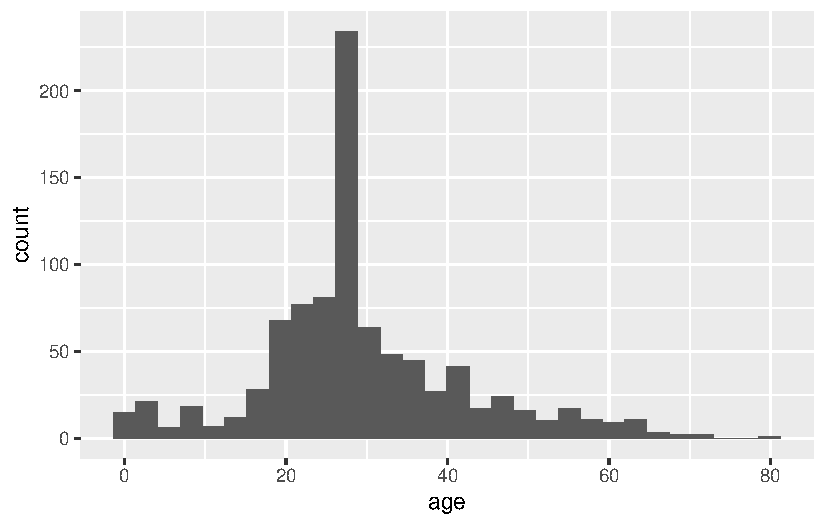
\includegraphics{FinalProject_files/figure-pdf/unnamed-chunk-10-1.pdf}

\begin{Shaded}
\begin{Highlighting}[]
\CommentTok{\# Bar chart showing that more females survived than males.}
\FunctionTok{ggplot}\NormalTok{(train, }\FunctionTok{aes}\NormalTok{(survived)) }\SpecialCharTok{+}
  \FunctionTok{geom\_bar}\NormalTok{()}
\end{Highlighting}
\end{Shaded}

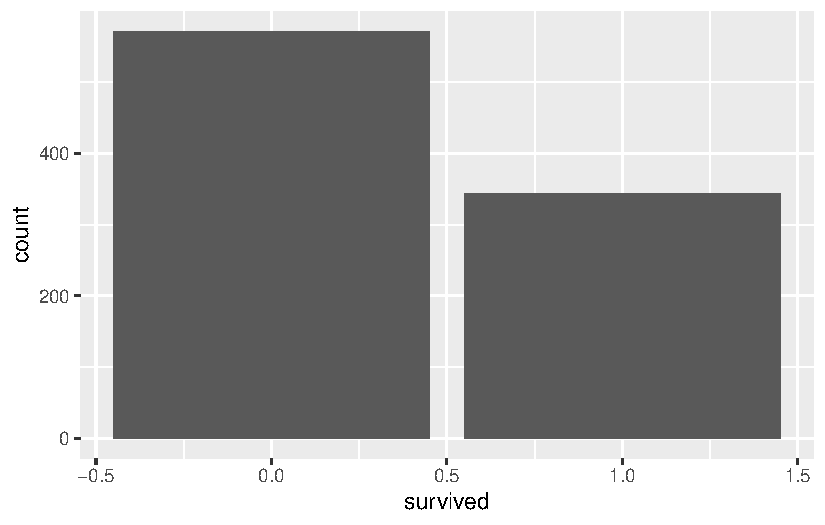
\includegraphics{FinalProject_files/figure-pdf/unnamed-chunk-10-2.pdf}

\begin{Shaded}
\begin{Highlighting}[]
\CommentTok{\# Bar chart showing that a higher number of people survived when they had less siblings on board.}
\FunctionTok{ggplot}\NormalTok{(train, }\FunctionTok{aes}\NormalTok{(sibsp, survived)) }\SpecialCharTok{+}
  \FunctionTok{geom\_bar}\NormalTok{(}\AttributeTok{stat=}\StringTok{\textquotesingle{}identity\textquotesingle{}}\NormalTok{)}
\end{Highlighting}
\end{Shaded}

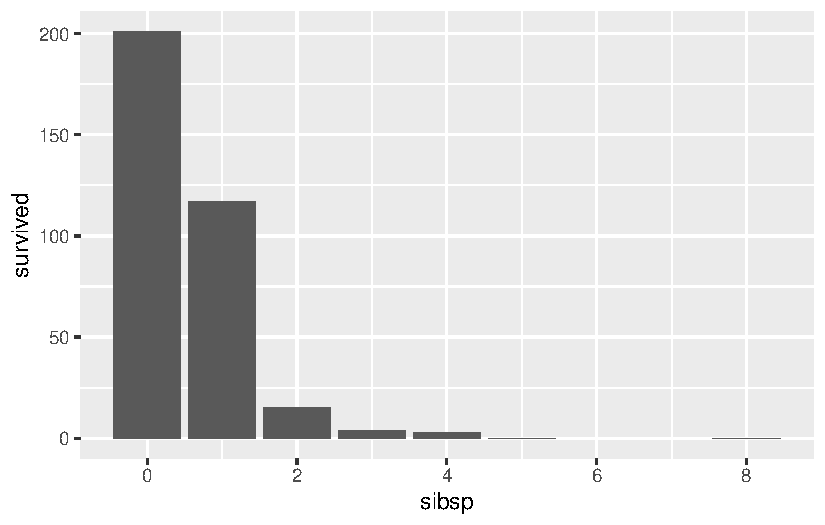
\includegraphics{FinalProject_files/figure-pdf/unnamed-chunk-10-3.pdf}

\begin{Shaded}
\begin{Highlighting}[]
\FunctionTok{ggplot}\NormalTok{(train, }\FunctionTok{aes}\NormalTok{(age, sibsp)) }\SpecialCharTok{+}
  \FunctionTok{geom\_point}\NormalTok{()}
\end{Highlighting}
\end{Shaded}

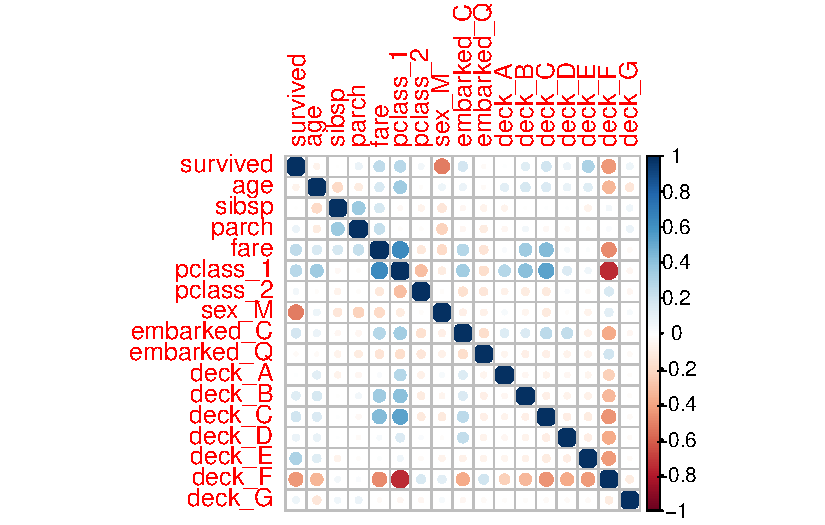
\includegraphics{FinalProject_files/figure-pdf/unnamed-chunk-10-4.pdf}

\begin{Shaded}
\begin{Highlighting}[]
\FunctionTok{ggplot}\NormalTok{(train, }\FunctionTok{aes}\NormalTok{(age, fare)) }\SpecialCharTok{+}
  \FunctionTok{geom\_point}\NormalTok{()}
\end{Highlighting}
\end{Shaded}

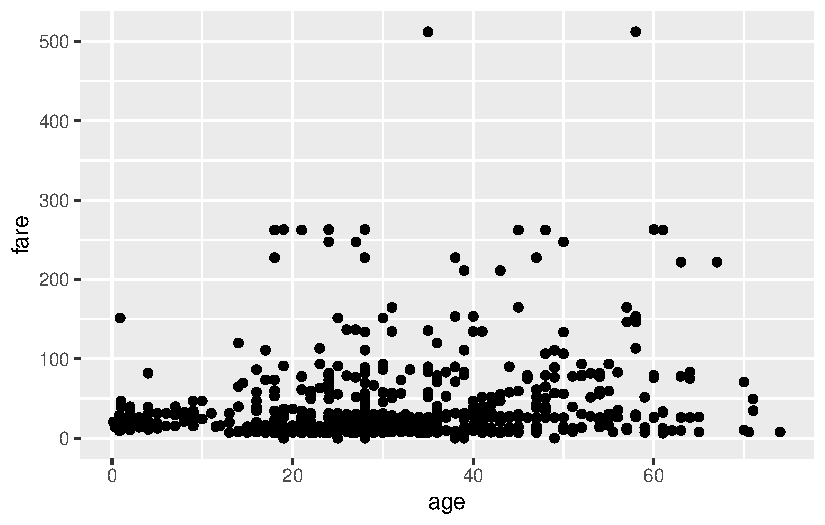
\includegraphics{FinalProject_files/figure-pdf/unnamed-chunk-10-5.pdf}

\begin{Shaded}
\begin{Highlighting}[]
\CommentTok{\#install.packages("psych")}
\FunctionTok{library}\NormalTok{(psych) }\CommentTok{\# Reference 4 to understand how this works}
\end{Highlighting}
\end{Shaded}

\begin{verbatim}
Warning: package 'psych' was built under R version 4.4.3
\end{verbatim}

\begin{verbatim}

Attaching package: 'psych'
\end{verbatim}

\begin{verbatim}
The following objects are masked from 'package:ggplot2':

    %+%, alpha
\end{verbatim}

\begin{Shaded}
\begin{Highlighting}[]
\FunctionTok{tetrachoric}\NormalTok{(train[, }\FunctionTok{c}\NormalTok{(}\StringTok{"survived"}\NormalTok{, }\StringTok{"sex\_M"}\NormalTok{)])}
\end{Highlighting}
\end{Shaded}

\begin{verbatim}
Call: tetrachoric(x = train[, c("survived", "sex_M")])
tetrachoric correlation 
         srvvd sex_M
survived  1.00      
sex_M    -0.75  1.00

 with tau of 
survived    sex_M 
    0.32    -0.37 
\end{verbatim}

\begin{Shaded}
\begin{Highlighting}[]
\FunctionTok{tetrachoric}\NormalTok{(train[, }\FunctionTok{c}\NormalTok{(}\StringTok{"survived"}\NormalTok{, }\StringTok{"pclass\_1"}\NormalTok{)])}
\end{Highlighting}
\end{Shaded}

\begin{verbatim}
Call: tetrachoric(x = train[, c("survived", "pclass_1")])
tetrachoric correlation 
         srvvd pcl_1
survived 1.00       
pclass_1 0.46  1.00 

 with tau of 
survived pclass_1 
    0.32     0.72 
\end{verbatim}

\begin{Shaded}
\begin{Highlighting}[]
\FunctionTok{tetrachoric}\NormalTok{(train[, }\FunctionTok{c}\NormalTok{(}\StringTok{"survived"}\NormalTok{, }\StringTok{"pclass\_2"}\NormalTok{)])}
\end{Highlighting}
\end{Shaded}

\begin{verbatim}
Call: tetrachoric(x = train[, c("survived", "pclass_2")])
tetrachoric correlation 
         srvvd pcl_2
survived 1.00       
pclass_2 0.08  1.00 

 with tau of 
survived pclass_2 
    0.32     0.83 
\end{verbatim}

\begin{Shaded}
\begin{Highlighting}[]
\CommentTok{\#install.packages("rcompanion")}
\FunctionTok{library}\NormalTok{(rcompanion) }\CommentTok{\# Reference 4 to understand how this works.}
\end{Highlighting}
\end{Shaded}

\begin{verbatim}
Warning: package 'rcompanion' was built under R version 4.4.3
\end{verbatim}

\begin{verbatim}

Attaching package: 'rcompanion'
\end{verbatim}

\begin{verbatim}
The following object is masked from 'package:psych':

    phi
\end{verbatim}

\begin{Shaded}
\begin{Highlighting}[]
\FunctionTok{cramerV}\NormalTok{(train}\SpecialCharTok{$}\NormalTok{survived, train}\SpecialCharTok{$}\NormalTok{sex)}
\end{Highlighting}
\end{Shaded}

\begin{verbatim}
Cramer V 
  0.5345 
\end{verbatim}

\begin{Shaded}
\begin{Highlighting}[]
\NormalTok{cor\_matrix }\OtherTok{\textless{}{-}} \FunctionTok{cor}\NormalTok{(train)}\CommentTok{\#[,1]}

\FunctionTok{library}\NormalTok{(corrplot)}
\end{Highlighting}
\end{Shaded}

\begin{verbatim}
corrplot 0.95 loaded
\end{verbatim}

\begin{Shaded}
\begin{Highlighting}[]
\FunctionTok{corrplot}\NormalTok{(cor\_matrix, }\AttributeTok{method =} \StringTok{"circle"}\NormalTok{)}
\end{Highlighting}
\end{Shaded}

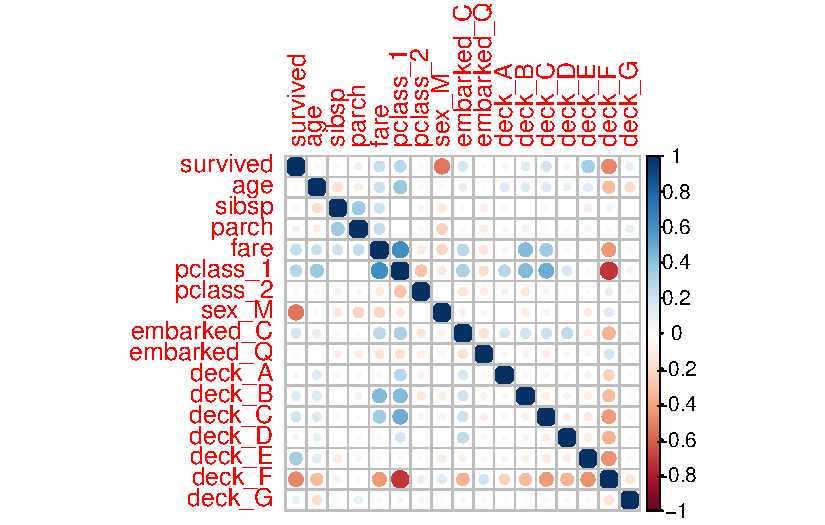
\includegraphics{FinalProject_files/figure-pdf/unnamed-chunk-10-6.pdf}

\section{III. Model Development
Process}\label{iii.-model-development-process}

Build an appropriate model to predict probability of survival. And of
course, create the train data set which contains 70\% of the data and
use set.seed (1023). The remaining 30\% will be your test data set.
Investigate the data and combine the level of categorical variables if
needed and drop variables. For example, you can passenger name, cabin,
etc..

\section{IV. Model Performance
Testing}\label{iv.-model-performance-testing}

Use the test data set to assess the model performances. Here, build the
best model by using appropriate selection method. You may compare the
performance of the best two logistic or other classification model
selected. Apply remedy measures as applicable (transformation, etc.)
that helps satisfy the assumptions of your particular model. Deeply
investigate unequal variances and multicollinearity if warranted.

\section{V. Challenger Models}\label{v.-challenger-models}

Build an alternative model based on one of the following approaches to
predict survival as applicable:logistic regression, decision tree, NN,
or SVM, Poisson regression or negative binomial. Check the applicable
model assumptions. Apply in-sample and out-of-sample testing, back
testing and review the comparative goodness of fit of the candidate
models. Describe step by step your procedure to get to the best model
and why you believe it is fit for purpose.

\section{VI. Model Limitation and
Assumptions}\label{vi.-model-limitation-and-assumptions}

Based on the performances on both train and test data sets, determine
your primary (champion) model and the other model which would be your
benchmark model. Validate your models using the test sample. Do the
residuals look normal? Does it matter given your technique? How is the
prediction performance using Pseudo Rˆ2, SSE, RMSE? Benchmark the model
against alternatives. How good is the relative fit? Are there any
serious violations of the logistic model assumptions? Has the model had
issues or limitations that the user must know? (Which assumptions are
needed to support the Champion model?)

\section{VII. Ongoing Model Monitoring
Plan}\label{vii.-ongoing-model-monitoring-plan}

How would you picture the model needing to be monitored, which
quantitative thresholds and triggers would you set to decide when the
model needs to be replaced? What are the assumptions that the model must
comply with for its continuous use?

In order to maintain the effectiveness of the model, we would need to
continue to test it on new data. Since the Titanic was a rare event, we
do not have a lot of new data to test on the model, but we can still be
prepared in case new data were to become available. The first step in
monitoring the model is to determine specific thresholds that we expect
the model to stay above. We would want the model to maintain certain
R\^{}2, RMSE, and MAE values in order to determine that the model is
working correctly. One of the biggest concerns with our model is data
drift. Since the Titanic sank over 100 years ago, the data that we are
using from the model may not align with today relevant to ship travel
today.

\section{VIII. Conclusion}\label{viii.-conclusion}

Summarize your results here. What is the best model for the data and
why?

\section{References}\label{references}

\section{Appendix}\label{appendix}

\subsection*{A:}\label{a}
\addcontentsline{toc}{subsection}{A:}

\phantomsection\label{refs}
\begin{CSLReferences}{1}{0}
\bibitem[\citeproctext]{ref-noaa2023}
National Oceanic and Atmospheric Administration (NOAA). (2023).
\emph{RMS titanic -- history and significance}.
\url{https://www.noaa.gov/office-of-general-counsel/gc-international-section/rms-titanic-history-and-significance}

\end{CSLReferences}




\end{document}
